\section{Methodology}
\label{sec:method}

CricketMind is built as one connected graph that answers two kinds of cricket question: a question about a specific video clip of a shot, and a question that is only text, with no video at all. Fig.~\ref{fig:arch-v2} shows the architecture; the node identifiers N1--N13 used below refer to it.

% Fig. 1 is fig_architecture.png, exported at 300 dpi from the TikZ source
% fig_architecture.tex (kept in this folder; render it with
% ../figure_blueprint/architecture_blueprint.tex after any edit).
% To use a redrawn Canva version instead, replace the file name below with
% Clip.png and check that the paper is still six pages.
\begin{figure*}[t]
  \centering
  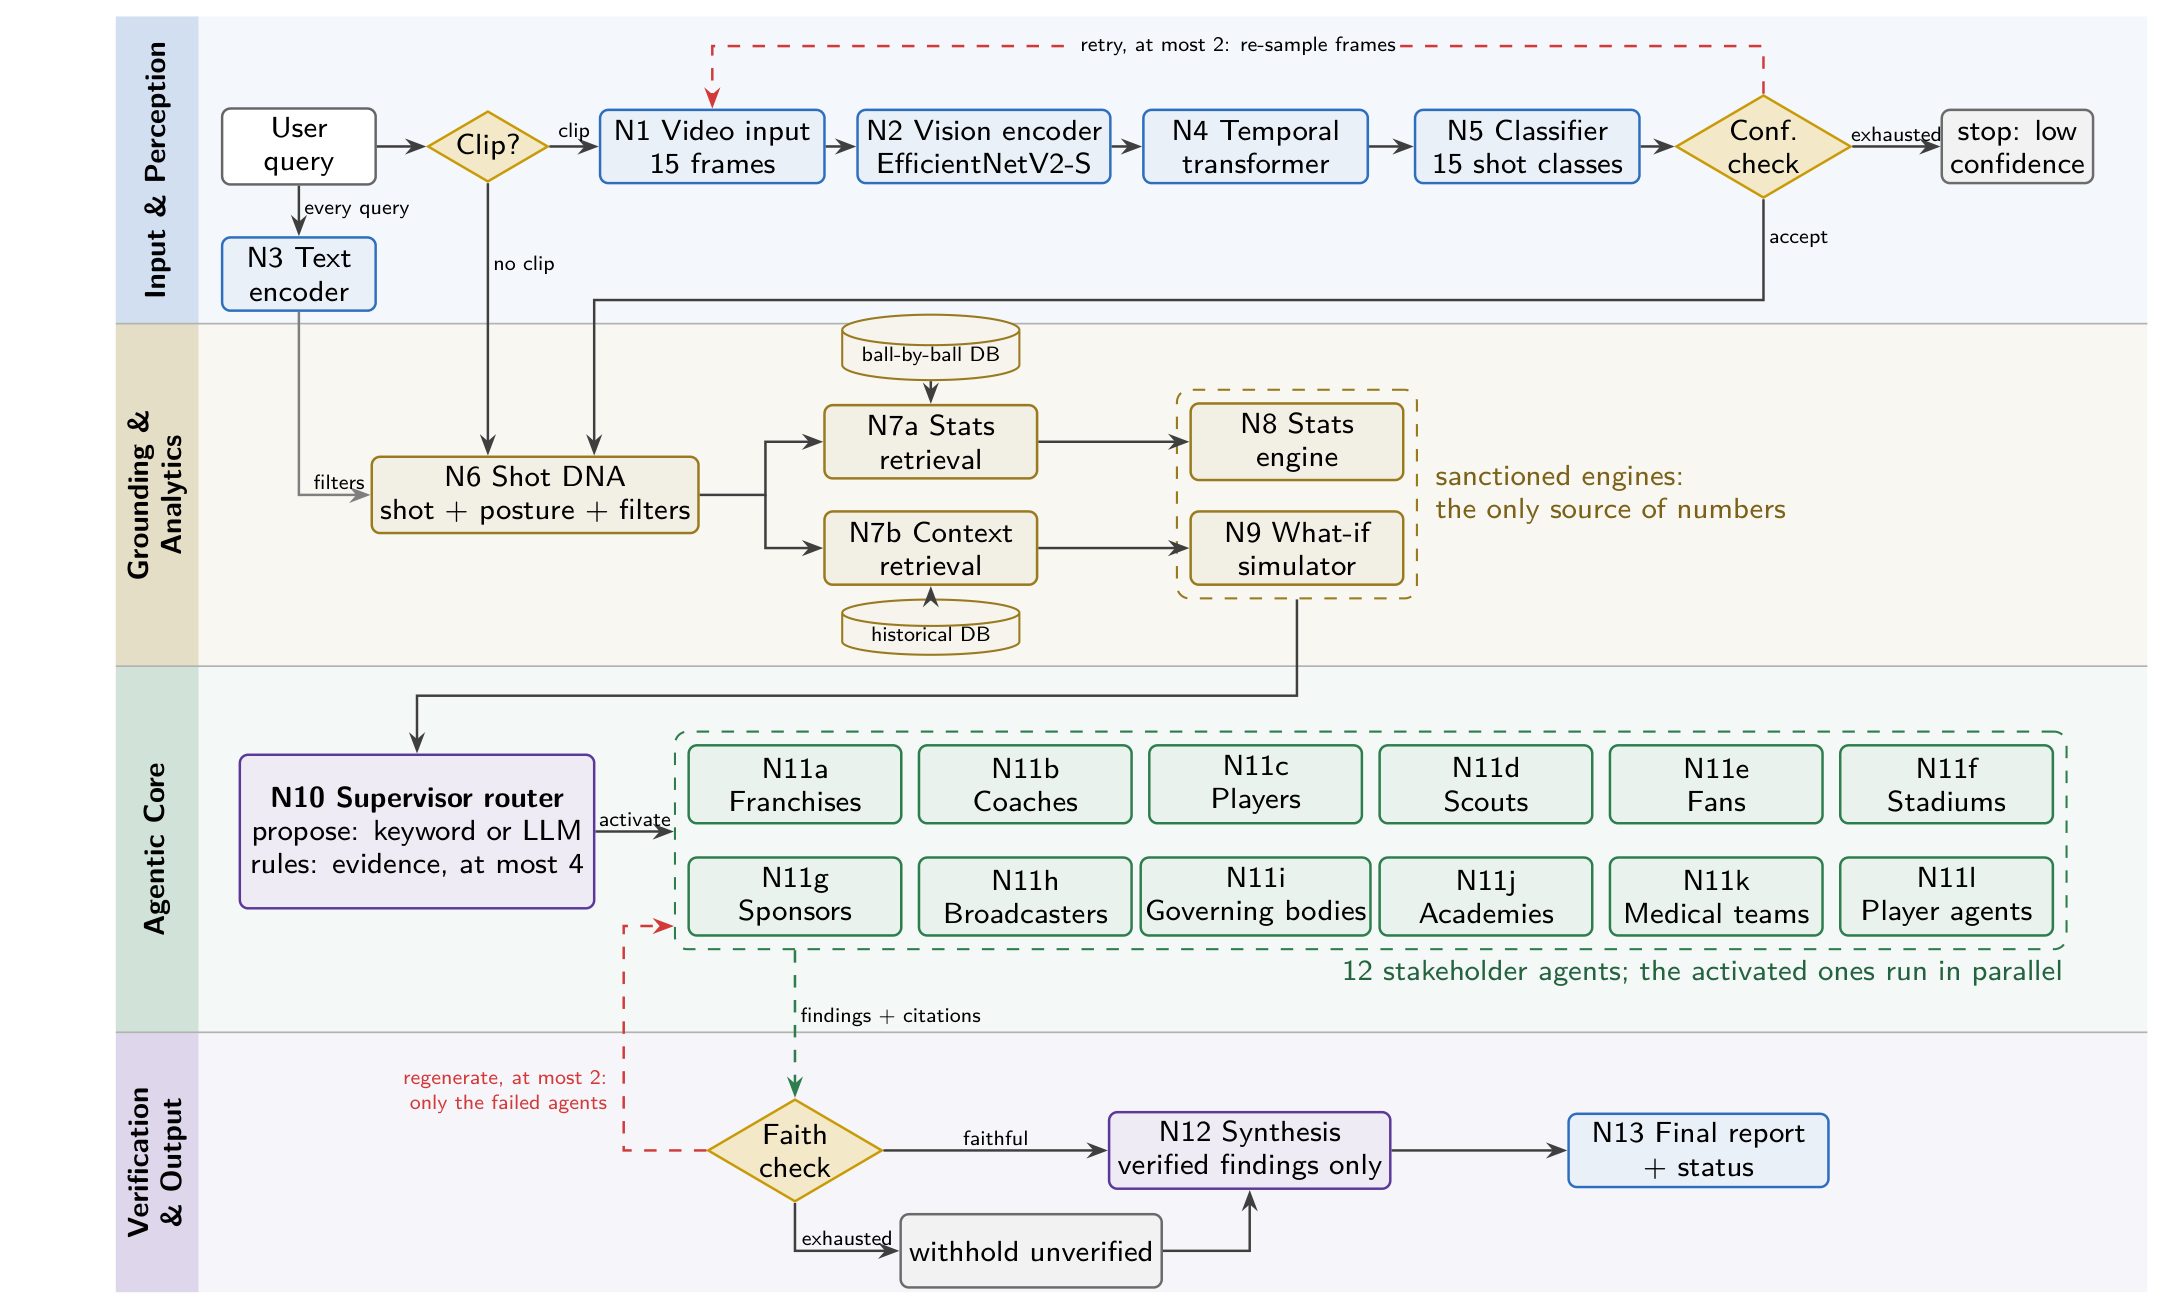
\includegraphics[width=\textwidth]{fig_architecture.png}
  \caption{The CricketMind architecture. A query carrying a clip enters the perception path (N1--N5); a text-only query bypasses it and reaches the Shot DNA (N6) directly. The text encoder (N3) runs on both paths. Red dashed edges are the two bounded correction loops: the confidence retry and the Faith Check regeneration.}
  \label{fig:arch-v2}
\end{figure*}

\subsection{Two Entry Paths and Perception}
When a query is submitted, the system first checks whether a video clip is attached. If it is, the clip is uniformly sampled into fifteen frames (N1), enough to capture the whole shot from the backlift to the follow-through without spending effort on near-identical frames. A vision encoder (N2, EfficientNetV2-S) turns each frame into a 1280-dimensional feature vector, and a small temporal transformer (N4, two layers, four heads) fuses the fifteen vectors. Because self-attention lets the first frame of the shot directly influence the last, the fused representation is designed to separate shots that look similar frame by frame but differ in the order and speed of motion, such as a sweep and a reverse sweep. A classifier head (N5) then predicts one of the fifteen shot classes of CricShot10k \cite{ref9} together with a confidence score.

A confidence gate adjudicates that prediction. A label with confidence of at least 0.70 is accepted. Below that, the system does not accept the result but re-samples the clip's frames and classifies again, at most twice; if the confidence is still too low, the query terminates with an explicit low-confidence status, before any agent is invoked, so an unreliable label is never passed forward silently. At the same time, and on both paths, a text encoder (N3) embeds the query and extracts the filters it implies---the player, the bowler type, the match phase, and any shots the question names---so the system knows which player, shot or situation is being asked about even when there is no video.

\subsection{The Shot DNA}
The accepted shot label, the query filters and posture measurements such as weight transfer, bat-face angle and stride length are combined into one structured record, the Shot DNA (N6). A text-only query skips the entire video path and arrives at this same record directly, carrying only the information taken from its own text. In that case the posture measurements are left out rather than filled in with a guess, because inventing a measurement that was never taken would quietly poison the very record that the rest of the system is built to trust. The Shot DNA is the only interface between perception and analysis: every later node reads it, and none touches the video again.

\subsection{Retrieval and the Sanctioned Engines}
The Shot DNA is used to search two separate indexes: a precise ball-by-ball index (N7a) that returns the specific deliveries matching the query, and a broader historical index (N7b) that returns career-level context, so the analysis is neither too narrow nor too general. Two shared calculation engines then take over. The statistics engine (N8) computes exact aggregates, such as strike rate and dismissal rate per shot, from the retrieved deliveries. The what-if simulator (N9) answers questions about hypothetical situations by Monte Carlo simulation, reporting how likely an outcome is together with a 95\% confidence interval. These two engines are the only parts of the system allowed to produce a number; their outputs form the \emph{sanctioned facts} of the query, and every other component must cite them rather than compute its own.

\subsection{Routing}
A supervisor router (N10) decides which of twelve specialised agents answer the query. Each agent serves one cricket stakeholder: franchises, coaches, players, scouts, fans, stadiums, sponsors, broadcasters, governing bodies, academies, medical teams and player agents. Routing has two stages. First, a router \emph{proposes} agents. The keyword router scores each agent by the words of its keyword list that appear in the query, plus two structural signals from the analytics: a low visual confidence, which suggests a technique question, and a large strike-rate spread between shots, which suggests a tactical one. The language-model router instead asks a language model, which sees each agent's stakeholder name and keyword list and must reply, under a fixed JSON schema, with one to four agent identifiers from the registry. Second, fixed rules \emph{decide}, identically for either router: an agent whose cited facts do not exist for the query is removed, at most four agents are kept, and if none remain a default pair (Coaches and Players) answers. On a text-only query, for instance, the agents focused on personal technique and player development are removed, because their answers would depend on posture measurements that were never taken; the report is shorter but still fully backed by evidence. Because the rules follow the proposal, the language model can suggest which agents answer but cannot activate an agent whose evidence does not exist, nor exceed the cap.

\subsection{Citation Contract and the Faith Check}
Every agent returns its answer together with a citation record that lists each figure it uses and the sanctioned fact it was taken from. Before any answer is shown to the user, the Faith Check compares every cited figure with the value the engines actually produced. If an agent cites a figure that does not match, only that agent is sent back to regenerate its answer from the real evidence, at most twice; if it still fails, its finding is withheld and the report states that it was withheld. The gate therefore guarantees that no cited figure contradicting the engines reaches the user. It checks citations, not prose: a correct figure attributed to the wrong subject, or a figure an agent states without citing it, lies outside what it can detect, which is why the citation record must be enforced on the agents' output format.

\subsection{Synthesis}
Finally, the verified findings are combined into one readable report that directly answers the user's question (N12), and the report is returned with a status (N13): \texttt{ok}, \texttt{low\_confidence} if the clip could not be classified, or \texttt{unverified\_claims\_dropped} if a finding was withheld.

\subsection{Implementation Status}
We implement the architecture as a LangGraph state graph with one node per component of Fig.~\ref{fig:arch-v2}, 30 nodes in total. In the implementation evaluated in this paper, node bodies are deterministic stand-ins. No video is decoded: the classifier returns a configurable label and confidence, which lets the confidence gate and the retry loop be exercised on demand. Retrieval operates over a small synthetic corpus of 150 deliveries and four historical records with known ground truth. The stakeholder agents generate their answers from templates over the sanctioned facts, emitting the same citation record that a language-model agent would be constrained to produce, and the report is composed from a template. The one exception is the router: alongside the keyword router we evaluate a language-model router, Qwen2.5-7B served locally through Ollama (Section~\ref{sec:routing}). Evaluating the accuracy of the perception front end is outside the scope of this paper. Values in the examples illustrate the flow of data and do not describe real match data.
